\section{多维随机变量及其函数分布}

抛两枚骰子，把第一枚的点数记为 $X$，第二枚记为 $Y$。要描述 $X$ 的分布，说“$1$ 到 $6$ 各占 $1/6$”就够了；$Y$ 也一样。可是“两枚点数之和是 $7$”的概率，单靠这两个分布算不出来——它取决于两个点数怎么搭配。同样，身高和体重各自都近似服从正态分布，但“身高超过 $180$ 且体重不足 $50$ 公斤”的概率，也不能由两个一维分布直接相乘得到。

两个随机变量放在一起研究时，需要的新对象是二维随机变量 $(X,Y)$，它取平面上的点，分布叫联合分布。下面的两张表最能说明“联合”比“各自”多出了什么。

\begin{center}
\begin{tikzpicture}[scale=1.0,font=\scriptsize]
  % ---------- 表 1 ----------
  \begin{scope}
    \draw[thick] (0,0) rectangle (2.2,2.2);
    \draw[gray!60] (1.1,0) -- (1.1,2.2);
    \draw[gray!60] (0,1.1) -- (2.2,1.1);
    \node at (0.55,1.65) {0.20};
    \node at (1.65,1.65) {0.30};
    \node at (0.55,0.55) {0.30};
    \node at (1.65,0.55) {0.20};
    \draw[gray!60] (2.45,0) -- (2.45,2.2);
    \node at (2.85,1.65) {0.50};
    \node at (2.85,0.55) {0.50};
    \draw[gray!60] (0,-0.45) -- (2.2,-0.45);
    \node at (0.55,-0.80) {0.50};
    \node at (1.65,-0.80) {0.50};
    \node at (0.55,2.50) {$Y=0$};
    \node at (1.65,2.50) {$Y=1$};
    \node at (-0.55,1.65) {$X=0$};
    \node at (-0.55,0.55) {$X=1$};
    \node[gray!60!black] at (2.85,2.50) {行和};
    \node[gray!60!black] at (-0.55,-0.80) {列和};
  \end{scope}
  % ---------- 表 2 ----------
  \begin{scope}[xshift=5.6cm]
    \draw[thick] (0,0) rectangle (2.2,2.2);
    \draw[gray!60] (1.1,0) -- (1.1,2.2);
    \draw[gray!60] (0,1.1) -- (2.2,1.1);
    \node at (0.55,1.65) {0.25};
    \node at (1.65,1.65) {0.25};
    \node at (0.55,0.55) {0.25};
    \node at (1.65,0.55) {0.25};
    \draw[gray!60] (2.45,0) -- (2.45,2.2);
    \node at (2.85,1.65) {0.50};
    \node at (2.85,0.55) {0.50};
    \draw[gray!60] (0,-0.45) -- (2.2,-0.45);
    \node at (0.55,-0.80) {0.50};
    \node at (1.65,-0.80) {0.50};
    \node at (0.55,2.50) {$Y=0$};
    \node at (1.65,2.50) {$Y=1$};
    \node at (-0.55,1.65) {$X=0$};
    \node at (-0.55,0.55) {$X=1$};
  \end{scope}
\end{tikzpicture}
\par\vspace{2pt}
{\footnotesize\itshape 两张表的行和、列和都是 $0.5$，所以 $X$、$Y$ 各自的分布完全一样；格子里的数却不同。表 1 中 $X,Y$ 更容易取到相同的值（$P(X=Y)=0.40$），表 2 中四个格子等可能（$P(X=Y)=0.50$）。边缘分布只保留了“各自怎么分布”，丢掉了“如何搭配”。}
\end{center}

这两张表也预告了独立性：表 2 的每个格子都等于对应行和乘列和，表 1 则不是。本章先给出联合分布的三种写法（分布函数、分布律、概率密度），再从联合分布里读出边缘分布与条件分布，然后讨论独立性；后半部分处理 $(X,Y)$ 的函数 $g(X,Y)$——和、极值，以及一般的变量替换。三维、$n$ 维的提法完全平行，只是记号更长。

\subsection{联合分布函数}

\begin{mydef}{联合分布函数}{joint-cdf}
设 $X,Y$ 是定义在同一样本空间上的随机变量，称
\[
F(x,y)=P\bigl((X\le x)\cap(Y\le y)\bigr)=P(X\le x,\;Y\le y),\qquad (x,y)\in\mathbb R^2
\]
为 $(X,Y)$ 的联合分布函数，简称联合分布。$n$ 维时把 $F$ 写成 $F(x_1,\dots,x_n)=P(X_1\le x_1,\dots,X_n\le x_n)$。
\end{mydef}

$F(x,y)$ 是“点 $(X,Y)$ 落在左下角无穷矩形 $(-\infty,x]\times(-\infty,y]$ 里”的概率。$x$ 往右移，矩形变大，所以 $F$ 关于 $x$ 单调不减；关于 $y$ 同理。四个极端位置给出边界值：
\[
F(-\infty,y)=F(x,-\infty)=0,\qquad F(+\infty,+\infty)=1 .
\]
这里 $F(-\infty,y)$ 指 $x\to-\infty$ 时的极限；“事件 $\{X\le -\infty\}$”是空集，概率为 $0$。此外 $F$ 关于每个变量右连续：$F(x+0,y)=F(x,y)$，$F(x,y+0)=F(x,y)$。

单个 $F(x,y)$ 的数值没有直接意义，有意义的是两个角点之间的差。矩形
\[
D=\{x_1<X\le x_2,\; y_1<Y\le y_2\}
\]
上的概率要用四个角点拼出来：
\[
P\bigl((X,Y)\in D\bigr)=F(x_2,y_2)-F(x_1,y_2)-F(x_2,y_1)+F(x_1,y_1).
\]

\begin{center}
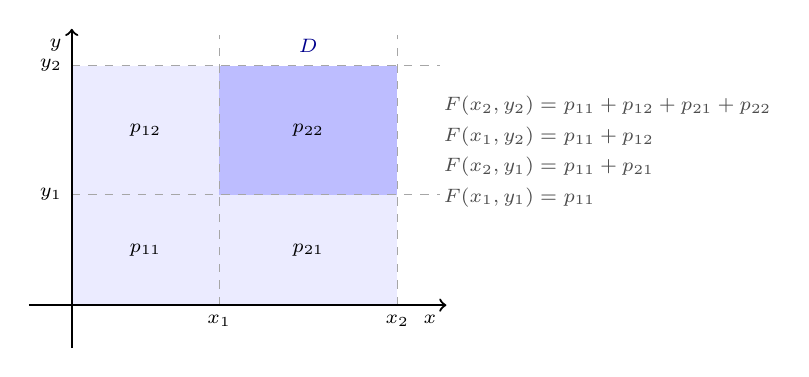
\begin{tikzpicture}[scale=0.78,font=\scriptsize]
  \fill[blue!8] (0,0) rectangle (2.4,1.8);
  \fill[blue!8] (2.4,0) rectangle (5.3,1.8);
  \fill[blue!8] (0,1.8) rectangle (2.4,3.9);
  \fill[blue!26] (2.4,1.8) rectangle (5.3,3.9);
  \draw[dashed,gray!70] (2.4,0) -- (2.4,4.4);
  \draw[dashed,gray!70] (5.3,0) -- (5.3,4.4);
  \draw[dashed,gray!70] (0,1.8) -- (6.0,1.8);
  \draw[dashed,gray!70] (0,3.9) -- (6.0,3.9);
  \draw[->,thick] (-0.7,0) -- (6.1,0) node[below left] {$x$};
  \draw[->,thick] (0,-0.7) -- (0,4.5) node[below left] {$y$};
  \node[below] at (2.4,0) {$x_1$};
  \node[below] at (5.3,0) {$x_2$};
  \node[left] at (0,1.8) {$y_1$};
  \node[left] at (0,3.9) {$y_2$};
  \node at (1.2,0.9) {$p_{11}$};
  \node at (3.85,0.9) {$p_{21}$};
  \node at (1.2,2.85) {$p_{12}$};
  \node at (3.85,2.85) {$p_{22}$};
  \node[blue!55!black] at (3.85,4.22) {$D$};
  \node[gray!60!black,align=left,anchor=west] at (5.9,2.5)
    {$F(x_2,y_2)=p_{11}+p_{12}+p_{21}+p_{22}$\\[3pt]
     $F(x_1,y_2)=p_{11}+p_{12}$\\[3pt]
     $F(x_2,y_1)=p_{11}+p_{21}$\\[3pt]
     $F(x_1,y_1)=p_{11}$};
\end{tikzpicture}
\par\vspace{2pt}
{\footnotesize\itshape 四条虚线把平面切成四块，$p_{22}$ 就是要求的那块。$F(x_2,y_2)$ 把四块全算上，减去左边一列 $p_{11}+p_{12}$，再减去下面一行 $p_{11}+p_{21}$；这时左下角 $p_{11}$ 被减了两次，于是加回一次，正好剩下 $p_{22}$。}
\end{center}

矩形公式还说明一件事：$F$ 不能随便给定，必须保证任意这样的矩形上的“四角组合”非负。离散型和连续型的联合分布都可以写成 $F$，所以 $F$ 是统一语言；但具体计算时，离散型看表、连续型用密度，比摆弄 $F$ 方便得多。

\subsection{离散型：联合分布律、边缘与条件}

若 $(X,Y)$ 只取有限或可列个点 $(x_i,y_j)$，记
\[
p_{ij}=P(X=x_i,\;Y=y_j),\qquad i,j=1,2,\dots
\]
则 $p_{ij}\ge 0$ 且 $\sum_i\sum_j p_{ij}=1$。这组数叫联合分布律。把它们排成表，行对应 $X$ 的取值，列对应 $Y$ 的取值，整张表的数加起来是 $1$。

按行求和、按列求和，就得到一维的边缘分布律：
\[
p_{i\cdot}=P(X=x_i)=\sum_{j}p_{ij},\qquad
p_{\cdot j}=P(Y=y_j)=\sum_{i}p_{ij}.
\]

\begin{center}
\begin{tikzpicture}[scale=0.95,font=\scriptsize]
  \fill[blue!10] (0,1.3) rectangle (3.9,2.6);
  \draw[thick] (0,0) rectangle (3.9,3.9);
  \draw[gray!60] (1.3,0) -- (1.3,3.9);
  \draw[gray!60] (2.6,0) -- (2.6,3.9);
  \draw[gray!60] (0,1.3) -- (3.9,1.3);
  \draw[gray!60] (0,2.6) -- (3.9,2.6);
  \node at (0.65,3.25) {0.10}; \node at (1.95,3.25) {0.15}; \node at (3.25,3.25) {0.05};
  \node at (0.65,1.95) {0.20}; \node at (1.95,1.95) {0.10}; \node at (3.25,1.95) {0.10};
  \node at (0.65,0.65) {0.05}; \node at (1.95,0.65) {0.05}; \node at (3.25,0.65) {0.20};
  % 行和
  \draw[gray!60] (4.1,0) -- (4.1,3.9);
  \node at (4.55,3.25) {0.30};
  \node at (4.55,1.95) {0.40};
  \node at (4.55,0.65) {0.30};
  % 列和
  \draw[gray!60] (0,-0.25) -- (3.9,-0.25);
  \draw[gray!60] (1.3,-1.3) -- (1.3,-0.25);
  \draw[gray!60] (2.6,-1.3) -- (2.6,-0.25);
  \node at (0.65,-0.78) {0.35};
  \node at (1.95,-0.78) {0.30};
  \node at (3.25,-0.78) {0.35};
  % 表头
  \node at (0.65,4.22) {$Y=0$};
  \node at (1.95,4.22) {$Y=1$};
  \node at (3.25,4.22) {$Y=2$};
  \node at (-0.62,3.25) {$X=0$};
  \node at (-0.62,1.95) {$X=1$};
  \node at (-0.62,0.65) {$X=2$};
  \node[gray!60!black] at (4.55,4.22) {行和};
  \node[gray!60!black] at (-0.62,-0.78) {列和};
  \node[gray!60!black,align=center] at (1.95,-1.75) {列和 $\Rightarrow$ $Y$ 的边缘分布};
  \node[gray!60!black,rotate=90,align=center] at (5.35,1.95) {行和 $\Rightarrow$ $X$ 的边缘分布};
\end{tikzpicture}
\par\vspace{2pt}
{\footnotesize\itshape 阴影是 $X=1$ 这一行。行和 $0.40$ 是 $P(X=1)$，把这一行的三个数除以 $0.40$，得到条件分布 $(0.50,0.25,0.25)$；行和与列和分别给出 $X$、$Y$ 的边缘分布。表里所有格子加起来是 $1$。}
\end{center}

有了表，很多概率可以直接数格子。例如 $P(X=Y)$ 是主对角线三个格子之和 $0.10+0.10+0.20=0.40$；$P(X+Y\le 1)$ 是满足条件的三格之和 $0.10+0.15+0.20=0.45$。

条件分布则是把一行（或一列）重新归一化。当 $P(X=x_i)=p_{i\cdot}>0$ 时，
\[
P(Y=y_j\mid X=x_i)=\frac{P(X=x_i,Y=y_j)}{P(X=x_i)}=\frac{p_{ij}}{p_{i\cdot}} .
\]
上式对固定的 $i$、把所有 $j$ 加起来等于 $1$，所以它确实是一个分布律。分母为 $0$ 的行不能条件化，这与一维条件概率要求 $P(B)>0$ 是一回事。

在连续型里，“固定一个变量”会得到密度而不是分布律，下一节先建立密度语言，再回到条件分布。

\subsection{连续型：联合密度与二维均匀分布}

\begin{mydef}{联合概率密度}{joint-density}
若存在非负可积函数 $f(x,y)$，使联合分布函数可写成
\[
F(x,y)=\int_{-\infty}^{x}\!\!\int_{-\infty}^{y}f(u,v)\,\mathrm dv\,\mathrm du ,
\]
则称 $f(x,y)$ 为 $(X,Y)$ 的联合概率密度。反过来，在 $f$ 连续的点上
\[
f(x,y)=\frac{\partial^2 F(x,y)}{\partial x\,\partial y}.
\]
\end{mydef}

密度满足 $f(x,y)\ge 0$、$\displaystyle\iint_{\mathbb R^2} f(x,y)\,\mathrm dx\,\mathrm dy=1$。任何区域上的概率是密度在该区域上的二重积分：
\[
P\bigl((X,Y)\in D\bigr)=\iint_D f(x,y)\,\mathrm dx\,\mathrm dy .
\]
密度是“单位面积上的概率”，不是概率；它的数值可以大于 $1$（只要面积足够小）。曲面 $z=f(x,y)$ 下的总体积为 $1$，区域 $D$ 上的概率就是 $D$ 上方那块的体积。

\begin{center}
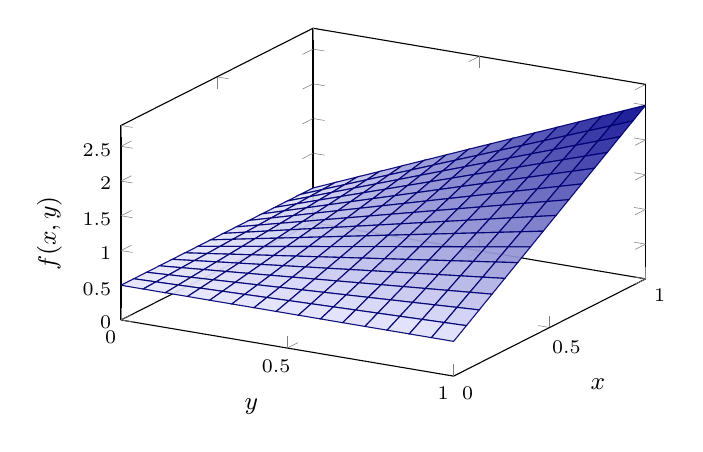
\begin{tikzpicture}
\begin{axis}[
  width=0.68\linewidth,height=6.0cm,
  view={120}{30}, x dir=reverse,
  xlabel={$x$},ylabel={$y$},zlabel={$f(x,y)$},
  xmin=0,xmax=1,ymin=0,ymax=1,zmin=0,zmax=2.8,
  xtick={0,0.5,1},ytick={0,0.5,1},ztick={0,0.5,1,1.5,2,2.5},
  tick label style={font=\scriptsize},
  label style={font=\small},
  colormap={dblue}{color=(blue!10) color=(blue!55!black)},
]
\addplot3[surf,shader=faceted,domain=0:1,domain y=0:1,samples=16,
  faceted color=blue!45!black,opacity=0.92]
  {(1/2)*(1+4*x*y)};
\end{axis}
\end{tikzpicture}
\par\vspace{2pt}
{\footnotesize\itshape 单位正方形上的密度 $f(x,y)=\frac12(1+4xy)$：左前角高度 $0.5$，右上角高度 $2.5$，曲面偏高说明那里的点更容易出现。概率等于曲面在相应区域上方的体积，整个方形上方的体积为 $1$。二维均匀分布的曲面是平的，概率就退化成面积乘常数。}
\end{center}

\begin{mydef}{二维均匀分布}{uniform-2d}
设 $G$ 是平面上的有界区域，面积为 $A>0$。若
\[
f(x,y)=\begin{cases}\dfrac{1}{A}, & (x,y)\in G,\\[4pt] 0, & (x,y)\notin G,\end{cases}
\]
则称 $(X,Y)$ 在 $G$ 上服从二维均匀分布。
\end{mydef}

均匀分布下密度是常数，概率只跟面积有关：
\[
P\bigl((X,Y)\in D\bigr)=\frac{\operatorname{area}(D\cap G)}{\operatorname{area}(G)} .
\]
例如在单位圆盘上均匀取点，落在一个张角为 $\theta$ 的扇形里的概率是 $\theta/(2\pi)$，与扇形朝哪个方向无关。要注意的是，均匀分布的边缘分布一般不均匀：圆盘上 $X$ 的密度中间高两边低，因为 $x$ 靠近中心时截得的弦更长。下一节就来讲这件事。

\subsection{边缘分布：把另一个变量积掉}

只关心 $X$ 时，把 $Y$ 的所有可能都算进来。分布函数层面是令 $y\to+\infty$：
\[
F_X(x)=P(X\le x)=F(x,+\infty),\qquad F_Y(y)=F(+\infty,y).
\]
连续型再对 $x$ 求导，得到边缘密度
\[
f_X(x)=\int_{-\infty}^{+\infty}f(x,y)\,\mathrm dy,\qquad
f_Y(y)=\int_{-\infty}^{+\infty}f(x,y)\,\mathrm dx .
\]
固定 $x$ 后，$f(x,y)$ 作为 $y$ 的函数是一条曲线，积分就是这条曲线下的面积。求 $f_Y$ 时对称处理，但积分变量换成 $x$。

\begin{center}
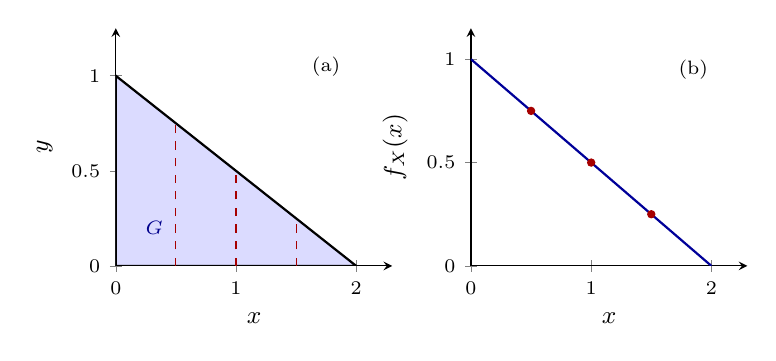
\begin{tikzpicture}
\begin{axis}[name=reg,width=0.42\linewidth,height=4.6cm,
  xmin=0,xmax=2.3,ymin=0,ymax=1.25,
  xlabel={$x$},ylabel={$y$},axis lines=left,
  xtick={0,1,2},ytick={0,0.5,1},
  tick label style={font=\scriptsize},label style={font=\small}]
\fill[blue!14] (axis cs:0,0) -- (axis cs:2,0) -- (axis cs:0,1) -- cycle;
\draw[thick] (axis cs:0,0) -- (axis cs:2,0) -- (axis cs:0,1) -- cycle;
\draw[dashed,red!65!black] (axis cs:0.5,0) -- (axis cs:0.5,0.75);
\draw[dashed,red!65!black] (axis cs:1.0,0) -- (axis cs:1.0,0.5);
\draw[dashed,red!65!black] (axis cs:1.5,0) -- (axis cs:1.5,0.25);
\node[font=\scriptsize,blue!55!black] at (axis cs:0.32,0.2) {$G$};
\node[font=\scriptsize] at (axis cs:1.75,1.05) {(a)};
\end{axis}
\begin{axis}[name=mar,at={(reg.east)},anchor=west,xshift=1.0cm,
  width=0.42\linewidth,height=4.6cm,
  xmin=0,xmax=2.3,ymin=0,ymax=1.15,
  xlabel={$x$},ylabel={$f_X(x)$},axis lines=left,
  xtick={0,1,2},ytick={0,0.5,1},
  tick label style={font=\scriptsize},label style={font=\small}]
\addplot[blue!60!black,thick,domain=0:2,samples=80]{1-x/2};
\addplot[only marks,mark=*,mark size=1.3pt,red!65!black]
  coordinates {(0.5,0.75) (1,0.5) (1.5,0.25)};
\node[font=\scriptsize] at (axis cs:1.85,0.95) {(b)};
\end{axis}
\end{tikzpicture}
\par\vspace{2pt}
{\footnotesize\itshape (a) 区域 $G$ 的顶点为 $(0,0),(2,0),(0,1)$，面积为 $1$，在 $G$ 上均匀分布时 $f\equiv 1$。三条红色虚线是固定 $x$ 时的竖截面，长度 $1-x/2$ 随 $x$ 变短。(b) 对应的边缘密度 $f_X(x)=1-x/2$，数值上恰好等于截面长度——这里因为 $f\equiv 1$ 且面积为 $1$。若密度不是常数，$f_X(x)$ 是截面上密度的积分，不是长度。}
\end{center}

上图中 $f_X(x)=\int_0^{1-x/2}1\,\mathrm dy=1-x/2$（$0<x<2$），$f_X$ 在别处为 $0$；同样 $f_Y(y)=\int_0^{2-2y}\mathrm dx=2-2y$（$0<y<1$）。两者在各自区间上积分都为 $1$，可以此自查。

两个容易出错的地方。第一是积分限：$f(x,y)\ne 0$ 的范围由支撑 $G$ 决定，$y$ 的上限常常是 $x$ 的函数，不能一律写 $-\infty$ 到 $+\infty$。第二是“积掉”不等于“忽略”：只有当 $X,Y$ 独立时，联合密度才等于两个边缘密度之积 $f=f_Xf_Y$；一般情况下 $f_X$ 与 $f_Y$ 乘起来是另一回事。

\subsection{条件分布：固定一个变量}

已知 $X=x$ 时，$Y$ 被限制在竖直线 $x=\text{常数}$ 上。把联合密度沿这条线切下一片 $y\mapsto f(x,y)$，它下方的面积正好是 $f_X(x)$。除以这块面积，曲线下的面积变成 $1$，就得到一条新的密度。

\begin{mydef}{条件概率密度}{cond-density}
设 $f_X(x)>0$，称
\[
f_{Y\mid X}(y\mid x)=\frac{f(x,y)}{f_X(x)}
\]
为条件 $X=x$ 下 $Y$ 的条件概率密度。对称地，
\[
f_{X\mid Y}(x\mid y)=\frac{f(x,y)}{f_Y(y)},\qquad f_Y(y)>0 .
\]
相应的条件分布函数为
\[
F_{Y\mid X}(y\mid x)=\int_{-\infty}^{y}\frac{f(x,t)}{f_X(x)}\,\mathrm dt .
\]
\end{mydef}

条件密度是对 $y$ 的密度：$\int_{-\infty}^{+\infty}f_{Y\mid X}(y\mid x)\,\mathrm dy=1$，积分变量是 $y$。因为分母只是常数，条件密度可以大于 $1$——它是“密度”，不是概率。离散型的条件分布律 $p_{ij}/p_{i\cdot}$ 与这里是一回事，只是求和换成了积分。

\begin{center}
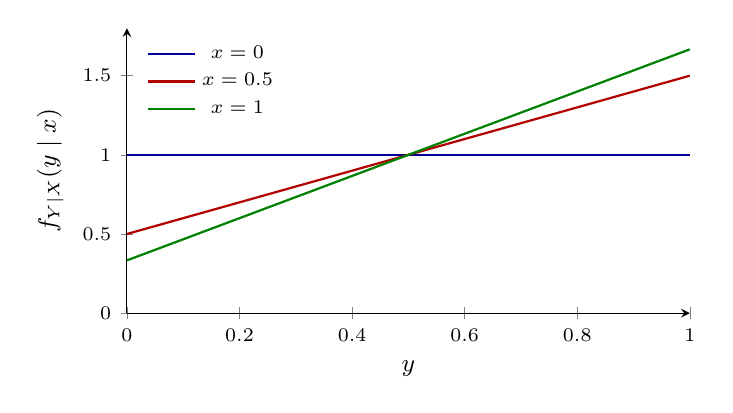
\begin{tikzpicture}
\begin{axis}[
  width=0.72\linewidth,height=5.2cm,
  xlabel={$y$},ylabel={$f_{Y\mid X}(y\mid x)$},
  xmin=0,xmax=1,ymin=0,ymax=1.8,
  domain=0:1,samples=100,
  axis lines=left,
  tick label style={font=\scriptsize},label style={font=\small},
  legend style={font=\scriptsize,draw=none,fill=none,
    at={(0.02,0.98)},anchor=north west},
]
\addplot[blue!60!black,thick]{1};
\addlegendentry{$x=0$}
\addplot[red!70!black,thick]{0.5+x};
\addlegendentry{$x=0.5$}
\addplot[green!50!black,thick]{(1+4*x)/3};
\addlegendentry{$x=1$}
\end{axis}
\end{tikzpicture}
\par\vspace{2pt}
{\footnotesize\itshape 仍用单位正方形上的 $f(x,y)=\frac12(1+4xy)$。固定 $x$ 切片再归一化：$x=0$ 时条件密度是常数 $1$，$Y$ 在 $(0,1)$ 上均匀；$x=\frac12$ 时它从 $0.5$ 升到 $1.5$；$x=1$ 时从 $\frac13$ 升到 $\frac53$。$x$ 越大，$Y$ 越容易取大值。三条曲线下的面积都是 $1$。如果 $X,Y$ 独立，三条曲线会完全重合。}
\end{center}

把定义式两边乘以 $f_X(x)$，得到密度的乘法公式
\[
f(x,y)=f_X(x)\,f_{Y\mid X}(y\mid x)=f_Y(y)\,f_{X\mid Y}(x\mid y),
\]
两个等号分别要求 $f_X(x)>0$、$f_Y(y)>0$。它在两个方向都有用：已知边缘密度和条件密度，可以拼出联合密度；已知联合密度，相除即得条件密度。离散型有完全平行的 $p_{ij}=p_{i\cdot}p_{j\mid i}$。

连续型有一个概念上的坎：$P(X=x)=0$，严格来说不能直接用一维条件概率定义 $P(Y\le y\mid X=x)$。工科教材的做法是把 $f_{Y\mid X}(\cdot\mid x)$ 当作 $h\to0$ 时 $\{x<X\le x+h\}$ 下条件分布的极限，计算上按上式处理即可，前提是 $f_X(x)>0$。

\subsection{独立性}

若知道 $X$ 的取值不改变 $Y$ 的分布，两个变量就“互不影响”。写成概率就是联合分布等于两个边缘分布相乘。

\begin{mydef}{随机变量的相互独立}{independence-ch3}
若对所有 $x,y$ 有
\[
F(x,y)=F_X(x)F_Y(y),
\]
则称 $X$ 与 $Y$ 相互独立。等价地，对任意事件 $A,B$ 有 $P(X\in A,\,Y\in B)=P(X\in A)P(Y\in B)$。
\end{mydef}

按分布类型写出具体判据：
\begin{itemize}
\item 离散型：对一切 $i,j$ 有 $p_{ij}=p_{i\cdot}\,p_{\cdot j}$。开头表 2 就是这种情形，表 1 则不是（$0.20\ne0.5\times0.5$）。
\item 连续型：$f(x,y)=f_X(x)f_Y(y)$ 几乎处处成立。只要除去面积为 $0$ 的集合后等式成立即可，个别线上不相等不影响。
\end{itemize}

判断连续型是否独立，有两个好用的线索。如果联合密度在矩形 $A\times B$ 上等于 $g(x)h(y)$，且支撑正好是 $A\times B$，那么独立，并且能直接读出 $f_X=g/\int_A g$、$f_Y=h/\int_B h$。反过来，如果密度的非零区域不是两个区间的直积（圆盘、三角形、被斜线切掉一角的方形），那一定不独立——因为条件分布会随另一个变量改变。

\begin{center}
\begin{tikzpicture}[font=\scriptsize,scale=1.1]
  \fill[blue!12] (0,0) rectangle (2,2);
  \draw[thick] (0,0) rectangle (2,2);
  \draw[red!65!black] (0.6,0) -- (0.6,2);
  \draw[red!65!black] (1.0,0) -- (1.0,2);
  \draw[red!65!black] (1.4,0) -- (1.4,2);
  \node at (1,2.3) {(a)};
  \node[align=center] at (1,-0.5) {矩形支撑：截面等长};
  % (b) 圆盘支撑
  \begin{scope}[xshift=5.2cm,yshift=1cm]
    \fill[blue!12] (0,0) circle (1);
    \draw[thick] (0,0) circle (1);
    \draw[red!65!black] (-0.6,{-sqrt(1-0.36)}) -- (-0.6,{sqrt(1-0.36)});
    \draw[red!65!black] (0,-1) -- (0,1);
    \draw[red!65!black] (0.6,{-sqrt(1-0.36)}) -- (0.6,{sqrt(1-0.36)});
    \node at (0,1.3) {(b)};
    \node[align=center] at (0,-1.5) {圆盘支撑：截面随 $x$ 变短};
  \end{scope}
\end{tikzpicture}
\par\vspace{2pt}
{\footnotesize\itshape 两图都是均匀分布，密度在各自的 $G$ 上为常数。(a) 每条竖截面的长度都相同，边缘密度是常数，联合密度可以分解成 $x$ 的函数乘 $y$ 的函数。(b) 竖截面长度为 $2\sqrt{1-x^2}$，中间长两边短，$f_X(x)=2\sqrt{1-x^2}/\pi$ 不是常数，条件分布也随 $x$ 变，所以 $X$ 与 $Y$ 不独立。}
\end{center}

独立性的几条常用性质：
\begin{enumerate}[label=(\arabic*),leftmargin=2.2em]
\item 独立变量的函数仍独立：若 $X,Y$ 独立，则 $g(X)$ 与 $h(Y)$ 独立，对任意（可测）函数 $g,h$ 成立。反过来一般不成立，除非 $g,h$ 都是可逆变换。
\item 独立时条件分布等于无条件分布：$f_{Y\mid X}(y\mid x)=f_Y(y)$，$p_{j\mid i}=p_{\cdot j}$。这正是“$X$ 的信息不影响 $Y$”的解析表达。
\item $n$ 个随机变量相互独立，指联合分布等于 $n$ 个边缘分布之积，等价于离散型对一切取值组合成立 $p_{i_1\cdots i_n}=\prod_k p^{(k)}_{i_k}$，连续型 $f=\prod_k f_k$ 几乎处处成立。独立变量中任意一部分也独立。
\item 两两独立不等于相互独立：三个变量两两独立只能保证每两个的联合分布分解，不能保证三者的联合分布等于三个边缘之积。
\item 独立一定不相关（协方差为 $0$，前提是方差存在），但不相关一般不推出独立；只有联合正态时两者才等价，见下一小节。另外，相关系数为 $0$ 只排除线性关系，像 $Y=X^2$（$X$ 关于 $0$ 对称）那样有强烈依赖但协方差为零的例子是存在的。
\end{enumerate}

\subsection{二维正态分布}

\begin{mydef}{二维正态分布}{bivariate-normal}
若 $(X,Y)$ 的联合密度为
\[
\begin{aligned}
f(x,y)={}&\frac{1}{2\pi\sigma_1\sigma_2\sqrt{1-\rho^2}}\\[2pt]
&\times\exp\!\left\{-\frac{1}{2(1-\rho^2)}
\left[\Bigl(\frac{x-\mu_1}{\sigma_1}\Bigr)^2+\Bigl(\frac{y-\mu_2}{\sigma_2}\Bigr)^2
-2\rho\,\frac{x-\mu_1}{\sigma_1}\cdot\frac{y-\mu_2}{\sigma_2}\right]\right\},
\end{aligned}
\]
其中 $\mu_1,\mu_2\in\mathbb R$，$\sigma_1,\sigma_2>0$，$-1<\rho<1$，则称 $(X,Y)$ 服从二维正态分布，记作
\[
(X,Y)\sim N(\mu_1,\mu_2;\sigma_1^2,\sigma_2^2;\rho).
\]
参数 $\mu_1,\mu_2$ 是中心位置，$\sigma_1,\sigma_2$ 控制两个方向的宽窄，$\rho$ 控制倾斜程度。
\end{mydef}

指数里是二次型，所以等密度线（$f$ 取常数的曲线）是一族同心椭圆。$\rho>0$ 时椭圆沿一、三象限方向拉长，$\rho<0$ 时沿二、四象限；$|\rho|$ 越大越扁，$\rho=0$ 时椭圆的两轴平行于坐标轴，退化成圆（当 $\sigma_1=\sigma_2$）。

\begin{center}
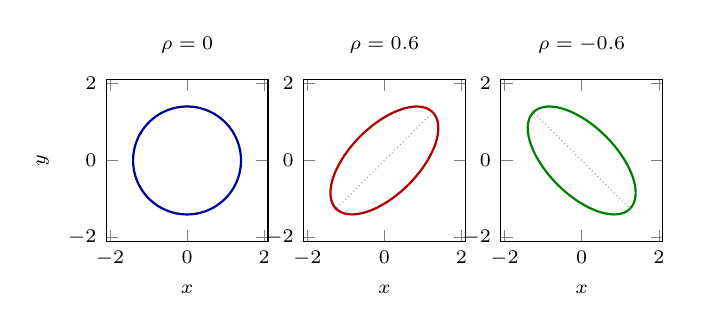
\begin{tikzpicture}
\begin{axis}[name=na,width=0.30\linewidth,height=4.2cm,
  xmin=-2.1,xmax=2.1,ymin=-2.1,ymax=2.1,
  xtick={-2,0,2},ytick={-2,0,2},axis equal image,
  tick label style={font=\scriptsize},
  title={\scriptsize $\rho=0$},
  xlabel={$x$},ylabel={$y$},label style={font=\scriptsize}]
\addplot[blue!60!black,thick,domain=0:360,samples=140]
  ({1.4*cos(x)},{1.4*sin(x)});
\end{axis}
\begin{axis}[name=nb,at={(na.east)},anchor=west,xshift=0.45cm,
  width=0.30\linewidth,height=4.2cm,
  xmin=-2.1,xmax=2.1,ymin=-2.1,ymax=2.1,
  xtick={-2,0,2},ytick={-2,0,2},axis equal image,
  tick label style={font=\scriptsize},
  title={\scriptsize $\rho=0.6$},
  xlabel={$x$},label style={font=\scriptsize}]
\addplot[red!70!black,thick,domain=0:360,samples=140]
  ({(1.77*cos(x)+0.885*sin(x))/1.4142},{(1.77*cos(x)-0.885*sin(x))/1.4142});
\addplot[gray!70,densely dotted,domain=-1.3:1.3]{x};
\end{axis}
\begin{axis}[name=nc,at={(nb.east)},anchor=west,xshift=0.45cm,
  width=0.30\linewidth,height=4.2cm,
  xmin=-2.1,xmax=2.1,ymin=-2.1,ymax=2.1,
  xtick={-2,0,2},ytick={-2,0,2},axis equal image,
  tick label style={font=\scriptsize},
  title={\scriptsize $\rho=-0.6$},
  xlabel={$x$},label style={font=\scriptsize}]
\addplot[green!50!black,thick,domain=0:360,samples=140]
  ({(0.885*cos(x)+1.77*sin(x))/1.4142},{(0.885*cos(x)-1.77*sin(x))/1.4142});
\addplot[gray!70,densely dotted,domain=-1.3:1.3]{-x};
\end{axis}
\end{tikzpicture}
\par\vspace{2pt}
{\footnotesize\itshape 三幅图画的是同一高度 $c=1.4$ 的等密度线（$\mu_1=\mu_2=0$，$\sigma_1=\sigma_2=1$）。$\rho=0$ 时是圆；$\rho=0.6$ 时椭圆沿 $y=x$ 拉长，长轴就是那条点线；$\rho=-0.6$ 时沿 $y=-x$ 拉长，方向正好相差 $90^\circ$。同一高度的椭圆越扁，说明该方向上概率衰减得越慢，$X$ 与 $Y$ 的线性关联越强。}
\end{center}

二维正态有几个必须记住的性质。

\begin{enumerate}[label=(\arabic*),leftmargin=2.2em]
\item 边缘分布仍是正态：$X\sim N(\mu_1,\sigma_1^2)$，$Y\sim N(\mu_2,\sigma_2^2)$，且与 $\rho$ 无关。反过来不成立：两个边缘都是正态，不能保证联合是二维正态。取 $X\sim N(0,1)$，另取与 $X$ 独立的 $S$，$P(S=1)=P(S=-1)=\frac12$，令 $Y=SX$，则 $Y\sim N(0,1)$，但 $(X,Y)$ 只落在两条直线 $y=\pm x$ 上，没有联合密度。
\item $X$ 与 $Y$ 相互独立的充要条件是 $\rho=0$。这也是“不相关”与“独立”等价的最常见场合。
\item 线性组合仍是正态：对不全为零的 $a,b$，
\[
aX+bY\sim N\Bigl(a\mu_1+b\mu_2,\; a^2\sigma_1^2+b^2\sigma_2^2+2ab\rho\sigma_1\sigma_2\Bigr).
\]
方差里的交叉项 $2ab\rho\sigma_1\sigma_2$ 不能丢；当 $\rho=0$ 时它才消失。
\item 条件分布也是正态：
\[
Y\mid X=x\;\sim\; N\!\left(\mu_2+\rho\frac{\sigma_2}{\sigma_1}(x-\mu_1),\;\sigma_2^2(1-\rho^2)\right).
\]
条件均值随 $x$ 线性变化，斜率是 $\rho\sigma_2/\sigma_1$；条件方差比 $\sigma_2^2$ 小，因为知道了 $X$ 就消掉一部分不确定性。
\end{enumerate}

\subsection{和的分布}

求 $Z=g(X,Y)$ 的分布，通用的做法只有一条：先算分布函数，再求导。以 $Z=X+Y$ 为例，
\[
F_Z(z)=P(X+Y\le z)=\iint_{x+y\le z}f(x,y)\,\mathrm dx\,\mathrm dy
=\int_{-\infty}^{+\infty}\!\!\left[\int_{-\infty}^{z-x}f(x,y)\,\mathrm dy\right]\mathrm dx .
\]
内层积分把“$X$ 取在 $x$ 附近时，$Y\le z-x$”的概率算出来，外层再把 $x$ 全部加起来。对 $z$ 求导（内层上限含 $z$），得
\[
f_Z(z)=\int_{-\infty}^{+\infty}f(x,z-x)\,\mathrm dx .
\]
若 $X,Y$ 独立，$f(x,z-x)=f_X(x)f_Y(z-x)$，于是
\[
\boxed{\;f_Z(z)=\int_{-\infty}^{+\infty}f_X(x)\,f_Y(z-x)\,\mathrm dx\;}
\]
这就是卷积公式。被积函数非零的范围由 $x$ 与 $z-x$ 各自必须落在支撑里这两条同时决定，所以积分往往要按 $z$ 分段。

\begin{center}
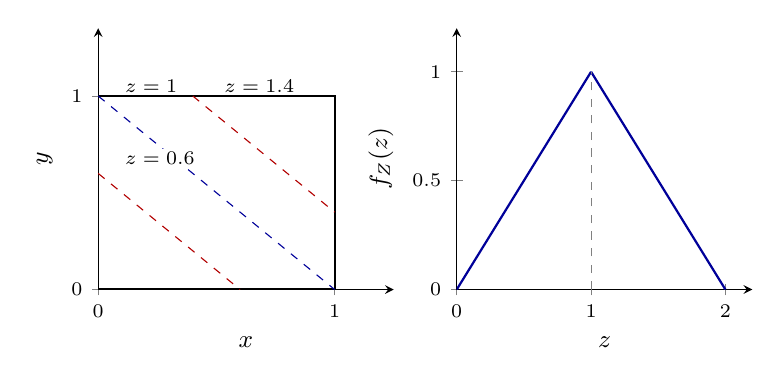
\begin{tikzpicture}
\begin{axis}[name=conc,width=0.44\linewidth,height=4.9cm,
  xmin=0,xmax=1.25,ymin=0,ymax=1.35,
  xlabel={$x$},ylabel={$y$},axis lines=left,
  xtick={0,1},ytick={0,1},
  tick label style={font=\scriptsize},label style={font=\small}]
\draw[thick] (axis cs:0,0) rectangle (axis cs:1,1);
\draw[dashed,red!70!black] (axis cs:0,0.6) -- (axis cs:0.6,0);
\draw[dashed,blue!60!black] (axis cs:0,1) -- (axis cs:1,0);
\draw[dashed,red!70!black] (axis cs:0.4,1) -- (axis cs:1,0.4);
\node[font=\scriptsize,anchor=west,fill=white,inner sep=1pt] at (axis cs:0.10,0.68) {$z=0.6$};
\node[font=\scriptsize,anchor=west,fill=white,inner sep=1pt] at (axis cs:0.10,1.05) {$z=1$};
\node[font=\scriptsize,anchor=west,fill=white,inner sep=1pt] at (axis cs:0.52,1.05) {$z=1.4$};
\end{axis}
\begin{axis}[name=dens,at={(conc.east)},anchor=west,xshift=0.8cm,
  width=0.44\linewidth,height=4.9cm,
  xmin=0,xmax=2.2,ymin=0,ymax=1.2,
  xlabel={$z$},ylabel={$f_Z(z)$},axis lines=left,
  xtick={0,1,2},ytick={0,0.5,1},
  tick label style={font=\scriptsize},label style={font=\small}]
\addplot[blue!60!black,thick,domain=0:1,samples=40]{x};
\addplot[blue!60!black,thick,domain=1:2,samples=40]{2-x};
\addplot[dashed,gray] coordinates {(1,0) (1,1)};
\end{axis}
\end{tikzpicture}
\par\vspace{2pt}
{\footnotesize\itshape 左：$X,Y$ 独立且都服从 $U(0,1)$，密度在单位正方形上为 $1$。$F_Z(z)$ 是直线 $x+y=z$ 左下方的面积；对 $z$ 求导，得到的是这条直线落在正方形里的线段在 $x$ 方向上的长度：$z<1$ 时为 $z$，$z>1$ 时为 $2-z$。右：长度先增后减，$f_Z$ 就是三角形，$z=1$ 处取最大值 $1$，总面积为 $1$。}
\end{center}

离散型是同样的“错位相乘再相加”：
\[
P(Z=z_k)=\sum_{i}P(X=x_i)\,P(Y=z_k-x_i),
\]
求和只保留 $z_k-x_i$ 确实是 $Y$ 的取值的那些项。

一个离散一个连续时，用全概率公式按离散变量的取值分组。若 $Y$ 离散、$P(Y=y_i)=p_i$，则
\[
F_Z(z)=\sum_i p_i\,P(X\le z-y_i)=\sum_i p_i\,F_X(z-y_i).
\]
这里用到了 $X$ 与 $Y$ 独立：只有独立时才可以把条件概率 $P(X\le z-y_i\mid Y=y_i)$ 换成 $F_X(z-y_i)$；否则要保留条件分布，写成 $\sum_i p_iF_{X\mid Y}(z-y_i\mid y_i)$。另外，$Z$ 一般既不是纯连续也不是纯离散的（它有正概率落在可列个点上，其余部分有密度），所以不能直接套卷积公式。

差、积、商的推导思路相同，都是先写成二重积分再换元。结果汇总在表里，使用前提都是 $X,Y$ 独立。

\begin{tablebox}{独立连续型随机变量函数的密度}
\centering
\begin{tabular}{ll}
\toprule
函数 & 密度 \\
\midrule
$Z=X+Y$ & $f_Z(z)=\displaystyle\int_{-\infty}^{+\infty}f_X(x)f_Y(z-x)\,\mathrm dx$ \\[11pt]
$Z=X-Y$ & $f_Z(z)=\displaystyle\int_{-\infty}^{+\infty}f_X(z+y)f_Y(y)\,\mathrm dy$ \\[11pt]
$Z=XY$ & $f_Z(z)=\displaystyle\int_{-\infty}^{+\infty}\frac{1}{|x|}f_X(x)f_Y\!\left(\frac{z}{x}\right)\mathrm dx$ \\[11pt]
$Z=X/Y$ & $f_Z(z)=\displaystyle\int_{-\infty}^{+\infty}|y|\,f_X(zy)f_Y(y)\,\mathrm dy$ \\[11pt]
\bottomrule
\end{tabular}
\end{tablebox}

积与商的公式里 $|x|$、$|y|$ 来自换元的雅可比，$x=0$、$y=0$ 的点由支撑自然排除。商的密度要求分母不为零；若 $Y$ 可能取 $0$，需要单独讨论。

\begin{conclusion}{分布的可加性}{additivity}
设 $X,Y$ 相互独立，则
\begin{enumerate}[label=(\arabic*),leftmargin=2.2em]
\item $X\sim B(n,p)$，$Y\sim B(m,p)$（注意 $p$ 相同）$\Rightarrow X+Y\sim B(n+m,p)$；
\item $X\sim P(\lambda_1)$，$Y\sim P(\lambda_2)$ $\Rightarrow X+Y\sim P(\lambda_1+\lambda_2)$；
\item $X\sim N(\mu_1,\sigma_1^2)$，$Y\sim N(\mu_2,\sigma_2^2)$ $\Rightarrow X+Y\sim N(\mu_1+\mu_2,\sigma_1^2+\sigma_2^2)$；
\item $X\sim\chi^2(n)$，$Y\sim\chi^2(m)$ $\Rightarrow X+Y\sim\chi^2(n+m)$。
\end{enumerate}
\end{conclusion}

这些结论对有限个相互独立的同类变量同样成立。可加性对参数有要求：两个二项分布的 $p$ 不同时，和不再是二项分布；两个均匀分布之和一般也不是均匀分布（正是上面的三角形）。

\subsection{极值分布}

最大值 $M=\max(X,Y)$ 与最小值 $m=\min(X,Y)$ 的分布，不要想着先写出密度。$\{M\le z\}$ 这个事件等价于“$X$ 和 $Y$ 都不超过 $z$”，而 $\{m>z\}$ 等价于“$X$ 和 $Y$ 都超过 $z$”，前者是交、后者也是交，正好能用独立性拆开。

\begin{conclusion}{最大值与最小值的分布}{max-min}
设 $X,Y$ 相互独立，分布函数分别为 $F_X,F_Y$，则
\[
F_{\max}(z)=F_X(z)F_Y(z),\qquad
F_{\min}(z)=1-\bigl[1-F_X(z)\bigr]\bigl[1-F_Y(z)\bigr].
\]
若 $X_1,\dots,X_n$ 独立同分布，分布函数为 $F$，则
\[
F_{\max}(z)=F^n(z),\qquad f_{\max}(z)=nF^{n-1}(z)f(z);
\]
\[
F_{\min}(z)=1-\bigl[1-F(z)\bigr]^n,\qquad f_{\min}(z)=n\bigl[1-F(z)\bigr]^{n-1}f(z).
\]
\end{conclusion}

最小值那条用对立事件推：$\{m>z\}=\{X>z,Y>z\}$，概率是 $[1-F_X(z)][1-F_Y(z)]$，取补即得。注意 $\{m\le z\}$ 并不等于 $\{X\le z\}\cup\{Y\le z\}$ 的简单相加，直接相加会把两者都小的情形算两遍。

\begin{center}
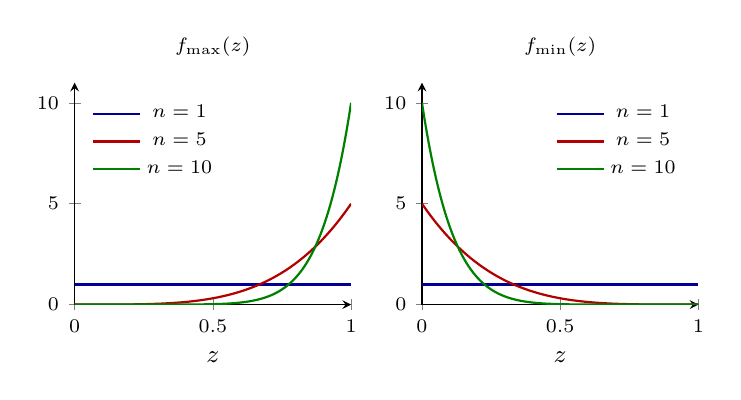
\begin{tikzpicture}
\begin{axis}[name=amax,width=0.42\linewidth,height=4.4cm,
  xmin=0,xmax=1,ymin=0,ymax=11,
  xlabel={$z$},title={\scriptsize $f_{\max}(z)$},axis lines=left,
  domain=0:1,samples=120,
  xtick={0,0.5,1},ytick={0,5,10},
  tick label style={font=\scriptsize},label style={font=\small},
  legend style={font=\scriptsize,draw=none,fill=none,
    at={(0.03,0.95)},anchor=north west}]
\addplot[blue!60!black,thick]{1};
\addlegendentry{$n=1$}
\addplot[red!70!black,thick]{5*x^4};
\addlegendentry{$n=5$}
\addplot[green!50!black,thick]{10*x^9};
\addlegendentry{$n=10$}
\end{axis}
\begin{axis}[name=amin,at={(amax.east)},anchor=west,xshift=0.9cm,
  width=0.42\linewidth,height=4.4cm,
  xmin=0,xmax=1,ymin=0,ymax=11,
  xlabel={$z$},title={\scriptsize $f_{\min}(z)$},axis lines=left,
  domain=0:1,samples=120,
  xtick={0,0.5,1},ytick={0,5,10},
  tick label style={font=\scriptsize},label style={font=\small},
  legend style={font=\scriptsize,draw=none,fill=none,
    at={(0.97,0.95)},anchor=north east}]
\addplot[blue!60!black,thick]{1};
\addlegendentry{$n=1$}
\addplot[red!70!black,thick]{5*(1-x)^4};
\addlegendentry{$n=5$}
\addplot[green!50!black,thick]{10*(1-x)^9};
\addlegendentry{$n=10$}
\end{axis}
\end{tikzpicture}
\par\vspace{2pt}
{\footnotesize\itshape 取 $X_i$ 独立同分布 $U(0,1)$。左：最大值的密度 $nz^{n-1}$，$n$ 越大越往 $z=1$ 挤——样本越多，最大值越接近上界，但永远不会超过它；峰值在 $z=1$ 处等于 $n$（密度可以大于 $1$）。右：最小值的密度 $n(1-z)^{n-1}$，形状是左边的镜像，向 $z=0$ 挤，峰值同样为 $n$。两条曲线都随 $n$ 增大变得越来越尖，这就是“极值分布”与单个变量分布形状不同的原因。}
\end{center}

指数分布的最小值有一个漂亮的结果。若 $X_1,\dots,X_n$ 独立且都服从 $\mathrm{Exp}(\lambda)$，则
\[
P(\min X_i>z)=\prod_{i=1}^{n}e^{-\lambda z}=e^{-n\lambda z},\qquad z>0,
\]
所以 $\min X_i\sim\mathrm{Exp}(n\lambda)$：$n$ 个独立指数“并联”，等待时间缩短为 $1/n$，速率相加。这个结论在可靠性里很常用，也是“指数分布无记忆性”的直接推论。

两个恒等式可以备查：
\[
\max(X,Y)=\frac{X+Y+|X-Y|}{2},\qquad
\min(X,Y)=\frac{X+Y-|X-Y|}{2}.
\]
逐点成立，所以取期望立刻得到 $E(\max)+E(\min)=E(X)+E(Y)$，求期望时能省一次积分。但求分布仍要走分布函数：最大值、最小值的密度一般不是 $f_Xf_Y$ 之类的乘积。

离散型没有密度，直接用分布律或分布函数列举。例如 $X,Y$ 只取 $0,1$ 时，$M=\max(X,Y)$ 在 $M=0$ 处只有 $(0,0)$ 一种来源，在 $M=1$ 处有其余三种来源，按格子加概率即可。

\subsection{变量替换与雅可比}

前面的卷积是从分布函数出发推出来的。如果一次要处理 $(X,Y)$ 的两个函数，或者函数形式复杂，更省事的办法是换元：把 $(x,y)$ 平面上的密度搬到 $(u,v)$ 平面上。

设 $U=g_1(X,Y)$，$V=g_2(X,Y)$，变换
\[
u=g_1(x,y),\qquad v=g_2(x,y)
\]
在密度非零的区域上有一阶连续偏导、是一一对应，反函数记为 $x=x(u,v)$、$y=y(u,v)$，且
\[
J=\frac{\partial(x,y)}{\partial(u,v)}
=\begin{vmatrix}
\dfrac{\partial x}{\partial u} & \dfrac{\partial x}{\partial v}\\[8pt]
\dfrac{\partial y}{\partial u} & \dfrac{\partial y}{\partial v}
\end{vmatrix}\ne 0 .
\]
则
\[
f_{U,V}(u,v)=f\bigl(x(u,v),\,y(u,v)\bigr)\,\bigl|J\bigr| ,
\]
在 $(u,v)$ 的像区域上成立，别处为 $0$。$|J|$ 是反函数在原像点处的面积伸缩因子：变换把面积放大了 $1/|J|$ 倍，密度就得乘 $|J|$ 才能保持总概率为 $1$。

\begin{center}
\begin{tikzpicture}[font=\scriptsize]
  % (a) 单位正方形
  \fill[blue!10] (0,0) rectangle (2,2);
  \draw[thick] (0,0) rectangle (2,2);
  \draw[gray!65] (1,0) -- (1,2);
  \draw[gray!65] (0,1) -- (2,1);
  \draw[->,thick] (2.15,0) -- (2.70,0) node[below] {$x$};
  \draw[->,thick] (1,2.15) -- (1,2.65) node[above] {$y$};
  \node at (1,-0.4) {(a) 面积 $1$};
  % 箭头
  \draw[->,very thick] (3.1,1) -- (4.3,1);
  \node[below,align=center] at (3.7,0.9) {$u=x+y$\\$v=x-y$};
  % (b) 菱形
  \fill[blue!10] (5.4,1) -- (6.4,2) -- (7.4,1) -- (6.4,0) -- cycle;
  \draw[thick] (5.4,1) -- (6.4,2) -- (7.4,1) -- (6.4,0) -- cycle;
  \draw[gray!65] (5.9,1.5) -- (6.9,0.5);
  \draw[gray!65] (5.9,0.5) -- (6.9,1.5);
  \draw[->,thick] (7.4,1) -- (7.9,1) node[right] {$u$};
  \draw[->,thick] (6.4,2) -- (6.4,2.5) node[above] {$v$};
  \node at (6.4,-0.4) {(b) 面积 $2$};
\end{tikzpicture}
\par\vspace{2pt}
{\footnotesize\itshape 左：单位正方形，灰线是 $x=\frac12$ 与 $y=\frac12$。右：像区域是顶点 $(0,0),(1,1),(2,0),(1,-1)$ 的菱形，两条灰线的像互相垂直地穿过中心。面积从 $1$ 变成 $2$，而
$J=\frac{\partial(x,y)}{\partial(u,v)}=-\frac12$，所以密度要乘 $\frac12$ 才守恒。图的形状会变，概率不会凭空增加。}
\end{center}

拿上面的变换做个完整计算。若 $(X,Y)$ 在单位正方形上均匀分布，$f\equiv1$，则
\[
f_{U,V}(u,v)=\begin{cases}
\dfrac12, & (u,v)\text{ 在菱形内},\\[4pt]
0, & \text{其他}.
\end{cases}
\]
菱形面积是 $2$，$\frac12\times2=1$，总概率对得上。再把 $v$ 积掉求 $f_U$：固定 $u\in(0,1)$，$v$ 的取值范围是 $|v|\le u$，长度 $2u$，所以 $f_U(u)=u$；对称地 $u\in(1,2)$ 时 $f_U(u)=2-u$。这正是上一节两个 $U(0,1)$ 之和的三角形密度——用换元法和用卷积法得到同一个结果，可以互相印证。

求单个函数 $Z=g(X,Y)$ 的密度时，可以人为补一个变量凑成二维变换，再积掉。比如取 $V=X$、$U=X+Y$，则 $x=v$、$y=u-v$，
\[
\left|\frac{\partial(x,y)}{\partial(u,v)}\right|
=\begin{vmatrix}0 & 1\\ 1 & -1\end{vmatrix}=1 ,
\]
于是 $f_{U,V}(u,v)=f(v,u-v)$，对 $v$ 积分就回到卷积公式。商的分布也这样做：取 $U=X/Y$、$V=Y$，反解 $x=uv$、$y=v$，雅可比为 $|v|$，即得表里的 $f_U(u)=\int|v|f(uv,v)\,\mathrm dv$。

如果变换不是一一对应，就要把原像分开算再相加。一维的典型例子是 $U=X^2$：$u>0$ 有两个原像 $x=\pm\sqrt u$，两个分支的雅可比分别是 $\frac{1}{2\sqrt u}$，所以
\[
f_U(u)=\frac{1}{2\sqrt u}\Bigl[f_X(\sqrt u)+f_X(-\sqrt u)\Bigr],\qquad u>0 .
\]
漏掉一个分支是这类题最常见的错误，做题时先画出变换后每个点有几个原像。

极坐标是最常用的非线性换元。令 $x=r\cos\theta$、$y=r\sin\theta$，则 $J=\frac{\partial(x,y)}{\partial(r,\theta)}=r$。对独立标准正态的 $(X,Y)$，
\[
f_{R,\Theta}(r,\theta)=\frac{1}{2\pi}e^{-r^2/2}\cdot r,\qquad r>0,\ 0<\theta<2\pi,
\]
它可以拆成只含 $r$ 的因子与只含 $\theta$ 的因子，所以 $R$ 与 $\Theta$ 独立，$\Theta$ 在 $(0,2\pi)$ 上均匀，$R^2\sim\mathrm{Exp}(1/2)$。这条推导说明二维正态的密度具有旋转对称性，也是“用均匀随机数生成正态随机数”一类算法的依据。

\newpage

\section{习题}

\subsection{本章速览}

\begin{itemize}
  \item \textbf{联合、边缘、条件的关系。} 联合分布完整描述 $(X,Y)$；边缘分布由联合分布“积掉”另一个变量得到，但反过来一般不能由两个边缘分布还原联合分布。离散型看表求和，连续型对密度积分。
  \item \textbf{条件分布仍是分布。} 离散型 $P(Y=y_j\mid X=x_i)=\dfrac{p_{ij}}{p_{i\cdot}}$；连续型 $f_{Y\mid X}(y\mid x)=\dfrac{f(x,y)}{f_X(x)}$（要求 $f_X(x)>0$）。条件密度对 $y$ 积分为 $1$，可据此求条件概率和条件期望。
  \item \textbf{独立性要处处成立。} 离散型需对所有 $i,j$ 有 $p_{ij}=p_{i\cdot}p_{\cdot j}$；连续型需 $f(x,y)=f_X(x)f_Y(y)$ 几乎处处成立。若联合密度的非零区域不是“矩形”（两个区间之积），则 $X,Y$ 必不独立。
  \item \textbf{和的分布用卷积。} 独立时 $f_{X+Y}(z)=\displaystyle\int_{-\infty}^{+\infty}f_X(x)f_Y(z-x)\,\mathrm dx$，关键是确定被积函数非零的 $x$ 范围。正态、泊松、二项、卡方分布具有可加性。
  \item \textbf{极值先求分布函数。} 独立时 $F_{\max}(z)=F_X(z)F_Y(z)$，$F_{\min}(z)=1-[1-F_X(z)][1-F_Y(z)]$；$n$ 个独立同分布时为 $F^n$ 与 $1-(1-F)^n$。先写分布函数再求导，不要直接猜密度。
  \item \textbf{变量替换要乘雅可比。} 若 $u=g_1(x,y),v=g_2(x,y)$ 有唯一反函数且 $J=\frac{\partial(x,y)}{\partial(u,v)}\neq0$，则 $f_{U,V}(u,v)=f\bigl(x(u,v),y(u,v)\bigr)|J|$；求单个函数的密度时，把另一个变量积掉。
\end{itemize}

\subsection{基础过关题}

\textbf{1.} 设二维离散型随机变量 $(X,Y)$ 的联合分布律为
\[
\begin{array}{c|ccc}
X\backslash Y & 0 & 1 & 2\\
\hline
0 & 0.12 & 0.08 & 0.10\\
1 & 0.18 & 0.12 & 0.10\\
2 & 0.10 & 0.20 & 0.00
\end{array}
\]
求：(1) $X,Y$ 的边缘分布律；(2) $P(X=Y)$ 与 $P(X+Y\leq 2)$；(3) 在 $X=1$ 的条件下 $Y$ 的条件分布律；(4) 判断 $X$ 与 $Y$ 是否独立。

\ifshowsolutions%
\boxed{\textbf{解}}
\textbf{思路：} 边缘分布按行、按列求和；事件概率把满足条件的格子概率相加；条件分布用该行概率除以行和；独立性只要找到一个格子不满足 $p_{ij}=p_{i\cdot}p_{\cdot j}$ 即可否定。

(1) 按行求和得 $X$ 的分布律
\[
P(X=0)=0.30,\qquad P(X=1)=0.40,\qquad P(X=2)=0.30.
\]
按列求和得 $Y$ 的分布律
\[
P(Y=0)=0.40,\qquad P(Y=1)=0.40,\qquad P(Y=2)=0.20.
\]

(2) $X=Y$ 的格子为 $(0,0),(1,1),(2,2)$，故
\[
P(X=Y)=0.12+0.12+0.00=0.24.
\]
满足 $X+Y\leq 2$ 的格子为 $(0,0),(0,1),(0,2),(1,0),(1,1),(2,0)$，故
\[
\begin{aligned}
P(X+Y\leq 2)&=0.12+0.08+0.10+0.18+0.12+0.10\\
&=0.70.
\end{aligned}
\]

(3) $P(X=1)=0.40$，于是
\[
\begin{aligned}
P(Y=0\mid X=1)&=\frac{0.18}{0.40}=0.45,\\
P(Y=1\mid X=1)&=\frac{0.12}{0.40}=0.30,\\
P(Y=2\mid X=1)&=\frac{0.10}{0.40}=0.25.
\end{aligned}
\]
三者之和为 $1$，计算正确。

(4) 虽然 $p_{00}=0.12=0.30\times0.40$，但
\[
p_{01}=0.08\neq 0.30\times0.40=0.12.
\]
只要有一个格子不成立就不独立，故 $X$ 与 $Y$ 不独立。

\[
\boxed{\begin{gathered}
\textbf{答案：}\quad \text{边缘分布如上；}\quad P(X=Y)=0.24,\quad P(X+Y\leq2)=0.70,\\
\text{条件分布为 }(0.45,0.30,0.25);\quad X,Y\text{ 不独立。}
\end{gathered}}
\]

\else \answerarea[10] \fi%
\textbf{2.} 设二维随机变量 $(X,Y)$ 的联合概率密度为
\[
f(x,y)=\begin{cases}
c(x+y), & 0<y<x<1,\\
0, & \text{其他}.
\end{cases}
\]
(1) 求常数 $c$；(2) 求边缘密度 $f_X(x),f_Y(y)$；(3) 求条件密度 $f_{Y\mid X}(y\mid x)$ 及 $P\!\left(Y<\frac{x}{2}\mid X=x\right)$；(4) 判断 $X$ 与 $Y$ 是否独立。

\ifshowsolutions%
\boxed{\textbf{解}}
\textbf{思路：} 先用规范性 $\iint f=1$ 定 $c$；求边缘密度时固定一个变量、在另一变量的实际范围内积分；条件密度由 $f/f_X$ 得到；条件概率对条件密度积分。

(1) 积分区域为 $0<x<1,\ 0<y<x$：
\[
\iint_D (x+y)\,\mathrm dy\,\mathrm dx
=\int_0^1\left(\int_0^x (x+y)\,\mathrm dy\right)\mathrm dx
=\int_0^1\left(x^2+\frac{x^2}{2}\right)\mathrm dx
=\frac32\cdot\frac13=\frac12.
\]
由 $c\cdot\frac12=1$ 得 $c=2$，即
\[
f(x,y)=2(x+y),\qquad 0<y<x<1.
\]

(2) 固定 $x\in(0,1)$，$y$ 的范围是 $(0,x)$：
\[
f_X(x)=\int_0^x 2(x+y)\,\mathrm dy
=2\left(x^2+\frac{x^2}{2}\right)=3x^2,\qquad 0<x<1.
\]
固定 $y\in(0,1)$，$x$ 的范围是 $(y,1)$：
\[
f_Y(y)=\int_y^1 2(x+y)\,\mathrm dx
=\left[x^2+2xy\right]_{x=y}^{x=1}
=1+2y-3y^2=(1-y)(3y+1),\qquad 0<y<1.
\]
验证：$\int_0^1(1+2y-3y^2)\,\mathrm dy=1+1-1=1$。

(3) 当 $0<x<1$ 时 $f_X(x)=3x^2>0$，故
\[
f_{Y\mid X}(y\mid x)=\frac{2(x+y)}{3x^2},\qquad 0<y<x.
\]
于是
\[
P\!\left(Y<\frac{x}{2}\mid X=x\right)
=\int_0^{x/2}\frac{2(x+y)}{3x^2}\,\mathrm dy
=\frac{1}{3x^2}\left[2xy+y^2\right]_0^{x/2}
=\frac{1}{3x^2}\left(x^2+\frac{x^2}{4}\right).
\]
注意 $2x\cdot\frac{x}{2}=x^2$，$\left(\frac{x}{2}\right)^2=\frac{x^2}{4}$，故概率为
\[
\frac{5x^2/4}{3x^2}=\frac{5}{12}.
\]

(4) 联合密度的非零区域是三角形 $0<y<x<1$，不是两个区间之积，故 $X,Y$ 不独立。也可取点验证：$f(\tfrac12,\tfrac14)=\tfrac32$，而
\[
f_X(\tfrac12)f_Y(\tfrac14)=\frac34\cdot\frac{21}{16}=\frac{63}{64}\neq\frac32.
\]

\boxed{\textbf{答案：}c=2;\ \text{边缘密度与条件密度如上；}P\!\left(Y<\frac{x}{2}\mid X=x\right)=\frac{5}{12};\ X,Y\text{ 不独立。}}

\else \answerarea[10] \fi%
\textbf{3.} 设 $X\sim U(0,1)$，在 $X=x\ (0<x<1)$ 的条件下 $Y\sim U(0,x^2)$。求：(1) $(X,Y)$ 的联合密度；(2) $Y$ 的边缘密度 $f_Y(y)$；(3) $E(Y)$（用条件期望与直接积分两种方法）；(4) $P(Y\leq \tfrac14)$。

\ifshowsolutions%
\boxed{\textbf{解}}
\textbf{思路：} 已知“边缘密度 $\times$ 条件密度”可还原联合密度；求 $f_Y$ 时固定 $y$，由 $y<x^2$ 解出 $x>\sqrt y$。计算期望时用重期望公式最快，再用直接积分核对。

(1) $f_X(x)=1\ (0<x<1)$，且当 $0<x<1$ 时
\[
f_{Y\mid X}(y\mid x)=\frac{1}{x^2},\qquad 0<y<x^2.
\]
由密度乘法公式
\[
f(x,y)=f_X(x)f_{Y\mid X}(y\mid x)=\frac{1}{x^2},\qquad 0<y<x^2<1.
\]
非零区域是 $0<x<1,\ 0<y<x^2$，其面积为 $\int_0^1 x^2\,\mathrm dx=\frac13$，而密度为 $1/x^2$，故总积分为 $\int_0^1\int_0^{x^2}x^{-2}\,\mathrm dy\,\mathrm dx=\int_0^1 1\,\mathrm dx=1$，规范性成立。

(2) 固定 $y\in(0,1)$。由 $0<y<x^2$ 得 $x>\sqrt y$，又 $x<1$，故 $x\in(\sqrt y,1)$：
\[
f_Y(y)=\int_{\sqrt y}^{1}\frac{1}{x^2}\,\mathrm dx
=\left[-\frac1x\right]_{\sqrt y}^{1}
=\frac{1}{\sqrt y}-1,\qquad 0<y<1.
\]
验证：$\int_0^1\left(y^{-1/2}-1\right)\mathrm dy=2-1=1$。

(3) 方法一（条件期望）：给定 $X=x$ 时 $Y\sim U(0,x^2)$，故
\[
E(Y\mid X=x)=\frac{x^2}{2},\qquad
E(Y)=E\!\left[\frac{X^2}{2}\right]=\frac{1}{2}\cdot\frac13=\frac16.
\]
方法二（直接积分）：
\[
E(Y)=\int_0^1 y\left(\frac{1}{\sqrt y}-1\right)\mathrm dy
=\int_0^1\left(y^{1/2}-y\right)\mathrm dy
=\frac23-\frac12=\frac16.
\]
两种方法一致。

(4)
\[
P\!\left(Y\leq\frac14\right)
=\int_0^{1/4}\left(\frac{1}{\sqrt y}-1\right)\mathrm dy
=\left[2\sqrt y-y\right]_0^{1/4}
=2\cdot\frac12-\frac14=\frac34.
\]

\[
\boxed{\begin{gathered}
\textbf{答案：}\quad f(x,y)=\frac{1}{x^2}\ (0<y<x^2<1),\qquad
f_Y(y)=\frac{1}{\sqrt y}-1\ (0<y<1),\\
E(Y)=\frac16,\qquad P\!\left(Y\leq\frac14\right)=\frac34.
\end{gathered}}
\]

\else \answerarea[10] \fi%
\textbf{4.} 设二维随机变量 $(X,Y)$ 的联合概率密度为
\[
f(x,y)=\begin{cases}
c\,\mathrm e^{-(x+2y)}, & 0<y<x,\\
0, & \text{其他}.
\end{cases}
\]
(1) 求 $c$；(2) 求边缘密度 $f_X(x),f_Y(y)$；(3) 判断 $X,Y$ 是否独立；(4) 求 $f_{X\mid Y}(x\mid y)$ 与 $E(X\mid Y=y)$，并求 $E(X)$。

\ifshowsolutions%
\boxed{\textbf{解}}
\textbf{思路：} 先按区域 $0<y<x<+\infty$ 积分定 $c$；边缘密度注意积分上限（$f_X$ 对 $y$ 从 $0$ 到 $x$，$f_Y$ 对 $x$ 从 $y$ 到 $+\infty$）。条件密度用 $f/f_Y$，条件期望对条件密度积分。

(1)
\[
\iint f\,\mathrm dy\,\mathrm dx
=c\int_0^{+\infty}\!\!\int_0^x \mathrm e^{-x-2y}\,\mathrm dy\,\mathrm dx
=c\int_0^{+\infty}\mathrm e^{-x}\cdot\frac{1-\mathrm e^{-2x}}{2}\,\mathrm dx.
\]
而
\[
\frac12\int_0^{+\infty}\left(\mathrm e^{-x}-\mathrm e^{-3x}\right)\mathrm dx
=\frac12\left(1-\frac13\right)=\frac13,
\]
故 $c\cdot\frac13=1$，即 $c=3$。

(2) 当 $x>0$ 时
\[
f_X(x)=\int_0^x 3\mathrm e^{-x-2y}\,\mathrm dy
=3\mathrm e^{-x}\cdot\frac{1-\mathrm e^{-2x}}{2}
=\frac32\left(\mathrm e^{-x}-\mathrm e^{-3x}\right).
\]
当 $y>0$ 时
\[
f_Y(y)=\int_y^{+\infty}3\mathrm e^{-x-2y}\,\mathrm dx
=3\mathrm e^{-2y}\cdot \mathrm e^{-y}=3\mathrm e^{-3y}.
\]
即 $Y\sim \Exp(3)$。验证 $f_X$ 的积分为 $\frac32(1-\frac13)=1$。

(3) 联合密度的非零区域 $0<y<x$ 不是矩形，故 $X,Y$ 不独立。也可由
\[
f(x,y)=3\mathrm e^{-x-2y}\neq \frac32\left(\mathrm e^{-x}-\mathrm e^{-3x}\right)\cdot 3\mathrm e^{-3y}=f_X(x)f_Y(y)
\]
（例如在 $x=y=1$ 处两边不相等）否定独立性。

(4) 当 $y>0$ 时 $f_Y(y)=3\mathrm e^{-3y}>0$，故
\[
f_{X\mid Y}(x\mid y)=\frac{3\mathrm e^{-x-2y}}{3\mathrm e^{-3y}}
=\mathrm e^{-(x-y)},\qquad x>y.
\]
即在 $Y=y$ 条件下 $X-y\sim \Exp(1)$，于是
\[
E(X\mid Y=y)=y+1.
\]
再由重期望公式及 $E(Y)=\frac13$，
\[
E(X)=E\bigl[E(X\mid Y)\bigr]=E(Y)+1=\frac13+1=\frac43.
\]

\[
\boxed{\begin{gathered}
\textbf{答案：}\quad c=3;\qquad
f_X(x)=\frac32\left(\mathrm e^{-x}-\mathrm e^{-3x}\right)\ (x>0),\\
f_Y(y)=3\mathrm e^{-3y}\ (y>0);\qquad X,Y\text{ 不独立};\\
f_{X\mid Y}(x\mid y)=\mathrm e^{-(x-y)}\ (x>y),\qquad E(X\mid Y=y)=y+1,\qquad E(X)=\frac43.
\end{gathered}}
\]

\else \answerarea[10] \fi%
\textbf{5.} 设 $(X,Y)$ 的联合分布律为
\[
\begin{array}{c|cc}
X\backslash Y & 0 & 1\\
\hline
0 & 0.1 & 0.2\\
1 & 0.3 & 0.4
\end{array}
\]
令 $U=X+Y$，$M=\max(X,Y)$。求：(1) $U$ 的分布律；(2) $M$ 的分布律；(3) 判断 $U$ 与 $M$ 是否独立。

\ifshowsolutions%
\boxed{\textbf{解}}
\textbf{思路：} 先列出 $(X,Y)$ 的四个取值及概率，再按 $U,M$ 的取值合并同类项；判断独立性时，找一对 $(u,m)$ 使联合概率不等于两个边缘概率之积。

四个基本结果：
\[
(0,0):0.1,\quad (0,1):0.2,\quad (1,0):0.3,\quad (1,1):0.4.
\]

(1) $U=X+Y$ 的可能取值为 $0,1,2$：
\[
P(U=0)=P(0,0)=0.1,
\]
\[
P(U=1)=P(0,1)+P(1,0)=0.2+0.3=0.5,
\]
\[
P(U=2)=P(1,1)=0.4.
\]
校验：$0.1+0.5+0.4=1$，且 $E(U)=0\times0.1+1\times0.5+2\times0.4=1.3$，与 $E(X)+E(Y)=0.7+0.6=1.3$ 一致，因为 $E(X+Y)=E(X)+E(Y)$ 恒成立。

(2) $M=\max(X,Y)$ 的可能取值为 $0,1$：
\[
P(M=0)=P(X=0,Y=0)=0.1,
\]
\[
P(M=1)=1-P(M=0)=0.9.
\]
也可直接相加：$P(0,1)+P(1,0)+P(1,1)=0.2+0.3+0.4=0.9$。

(3) 注意事件 $\{U=0\}=\{M=0\}=\{X=0,Y=0\}$，故
\[
P(U=0,M=0)=0.1,
\]
而
\[
P(U=0)P(M=0)=0.1\times0.1=0.01\neq0.1.
\]
所以 $U$ 与 $M$ 不独立。

\[
\boxed{\begin{gathered}
\textbf{答案：}\quad P(U=0)=0.1,\quad P(U=1)=0.5,\quad P(U=2)=0.4;\\
P(M=0)=0.1,\quad P(M=1)=0.9;\qquad U,M\text{ 不独立。}
\end{gathered}}
\]

\else \answerarea[10] \fi%

\subsection{综合提高题}
\textbf{6.} 设 $X\sim U(0,2)$，$Y\sim U(0,3)$，且 $X,Y$ 相互独立，$Z=X+Y$。求：(1) $f_Z(z)$；(2) $P(Z<2.5)$；(3) $E(Z)$ 与 $D(Z)$。

\ifshowsolutions%
\boxed{\textbf{解}}
\textbf{思路：} 用卷积公式。两个均匀密度的乘积为常数 $\frac16$，卷积值等于“满足 $0<z-x<3$ 的 $x$ 区间长度”乘以 $\frac16$，因此只需分段讨论区间长度。

(1) $f_X(x)=\frac12\ (0<x<2)$，$f_Y(y)=\frac13\ (0<y<3)$。由独立性，
\[
f_Z(z)=\int_{-\infty}^{+\infty}f_X(x)f_Y(z-x)\,\mathrm dx
=\frac16\int_0^2 \mathbf 1_{\{0<z-x<3\}}\,\mathrm dx.
\]
条件 $0<z-x<3$ 等价于 $z-3<x<z$，故积分区间为 $(0,2)\cap(z-3,z)$，其长度为
\[
\ell(z)=\begin{cases}
z, & 0<z<2,\\
2, & 2\leq z\leq 3,\\
5-z, & 3<z<5,\\
0, & \text{其他}.
\end{cases}
\]
于是
\[
f_Z(z)=\begin{cases}
\dfrac{z}{6}, & 0<z<2,\\[4pt]
\dfrac13, & 2\leq z\leq 3,\\[4pt]
\dfrac{5-z}{6}, & 3<z<5,\\[4pt]
0, & \text{其他}.
\end{cases}
\]
规范性校验：$\frac16\left(\int_0^2 z\,\mathrm dz+\int_2^3 2\,\mathrm dz+\int_3^5(5-z)\,\mathrm dz\right)=\frac16(2+2+2)=1$。

(2)
\[
P(Z<2.5)=\int_0^2\frac{z}{6}\,\mathrm dz+\int_2^{2.5}\frac13\,\mathrm dz
=\frac{2}{6}+\frac{1}{3}\cdot\frac12
=\frac13+\frac16=\frac12.
\]
这也与 $Z$ 的分布关于 $2.5$ 对称相符。

(3) 由期望与方差的可加性（独立性保证方差可加）：
\[
E(Z)=E(X)+E(Y)=1+\frac32=\frac52,
\]
\[
D(Z)=D(X)+D(Y)=\frac{2^2}{12}+\frac{3^2}{12}
=\frac13+\frac34=\frac{13}{12}.
\]

\boxed{\textbf{答案：}f_Z(z)=\begin{cases}\frac{z}{6},&0<z<2,\\ \frac13,&2\leq z\leq3,\\ \frac{5-z}{6},&3<z<5,\\ 0,&\text{其他};\end{cases}\quad P(Z<2.5)=\frac12;\quad E(Z)=\frac52,\ D(Z)=\frac{13}{12}.}

\else \answerarea[10] \fi%
\textbf{7.} 设 $X_1,X_2,X_3$ 相互独立，均服从 $U(0,1)$，记
\[
M=\max(X_1,X_2,X_3),\qquad m=\min(X_1,X_2,X_3).
\]
(1) 求 $M$ 的分布函数、密度与 $E(M)$；(2) 求 $m$ 的分布函数、密度与 $E(m)$；(3) 求 $(m,M)$ 的联合密度；(4) 用联合密度求 $E(M-m)$，并与 (1)(2) 的结果核对。

\ifshowsolutions%
\boxed{\textbf{解}}
\textbf{思路：} 极值问题先写分布函数：$\{M\leq z\}$ 等价于“每个都 $\leq z$”，$\{m>z\}$ 等价于“每个都 $>z$”。求联合密度时按“谁最大、谁最小、剩下一个落在中间”计数。

(1) 当 $0\leq z\leq1$ 时，由独立性
\[
F_M(z)=P(X_1\leq z,X_2\leq z,X_3\leq z)=z^3.
\]
故 $F_M(z)=0\ (z<0)$，$F_M(z)=1\ (z>1)$。求导得
\[
f_M(z)=3z^2,\qquad 0<z<1.
\]
于是
\[
E(M)=\int_0^1 z\cdot3z^2\,\mathrm dz=3\cdot\frac14=\frac34.
\]

(2) 当 $0\leq z\leq1$ 时，
\[
F_m(z)=1-P(m>z)=1-P(X_1>z,X_2>z,X_3>z)=1-(1-z)^3.
\]
求导得
\[
f_m(z)=3(1-z)^2,\qquad 0<z<1.
\]
于是
\[
E(m)=\int_0^1 3z(1-z)^2\,\mathrm dz
=3\left(\frac12-\frac23+\frac14\right)
=3\cdot\frac{1}{12}=\frac14.
\]

(3) 设 $0<u<v<1$。事件“$m\in\mathrm du,\ M\in\mathrm dv$”要求：三个变量中有一个取最小值（3 种选法），一个取最大值（2 种选法），剩下的一个落在 $(u,v)$ 内（长度 $v-u$）。由于每个 $X_i$ 的密度为 $1$，故
\[
f_{m,M}(u,v)\,\mathrm du\,\mathrm dv
=3\cdot 2\cdot(v-u)\,\mathrm du\,\mathrm dv,
\]
即
\[
f_{m,M}(u,v)=6(v-u),\qquad 0<u<v<1.
\]
规范性校验：
\[
\int_0^1\!\!\int_0^v 6(v-u)\,\mathrm du\,\mathrm dv
=\int_0^1 3v^2\,\mathrm dv=1.
\]

(4)
\[
E(M-m)=\int_0^1\!\!\int_0^v 6(v-u)^2\,\mathrm du\,\mathrm dv.
\]
内层积分
\[
\int_0^v 6(v-u)^2\,\mathrm du
=\left[-2(v-u)^3\right]_{u=0}^{u=v}=2v^3,
\]
故
\[
E(M-m)=\int_0^1 2v^3\,\mathrm dv=\frac12.
\]
而由 (1)(2)，$E(M)-E(m)=\frac34-\frac14=\frac12$，两者一致。

\[
\boxed{\begin{gathered}
\textbf{答案：}\quad F_M(z)=z^3,\quad f_M(z)=3z^2,\quad E(M)=\frac34;\\
F_m(z)=1-(1-z)^3,\quad f_m(z)=3(1-z)^2,\quad E(m)=\frac14;\\
f_{m,M}(u,v)=6(v-u)\ (0<u<v<1),\qquad E(M-m)=\frac12.
\end{gathered}}
\]

\else \answerarea[10] \fi%
\textbf{8.} 设 $X,Y$ 相互独立且都服从参数为 $1$ 的指数分布。令
\[
U=X+Y,\qquad V=\frac{X}{X+Y}.
\]
(1) 求 $(U,V)$ 的联合密度；(2) 求 $U,V$ 的边缘密度并判断独立性；(3) 指出 $U,V$ 各服从什么分布；(4) 求 $E(V)$。

\ifshowsolutions%
\boxed{\textbf{解}}
\textbf{思路：} 这是二重换元：先解出 $x,y$ 用 $u,v$ 表示，算雅可比行列式，再乘原联合密度。若结果能分解成“只含 $u$”与“只含 $v$”两个因子，则两者独立。

(1) 联合密度为
\[
f_{X,Y}(x,y)=\mathrm e^{-(x+y)},\qquad x>0,\ y>0.
\]
由 $u=x+y,\ v=\dfrac{x}{x+y}$ 反解：
\[
x=uv,\qquad y=u(1-v).
\]
由 $x>0,y>0$ 得 $u>0,\ 0<v<1$。雅可比行列式
\[
J=\frac{\partial(x,y)}{\partial(u,v)}
=\begin{vmatrix}
\dfrac{\partial x}{\partial u} & \dfrac{\partial x}{\partial v}\\[6pt]
\dfrac{\partial y}{\partial u} & \dfrac{\partial y}{\partial v}
\end{vmatrix}
=\begin{vmatrix}
v & u\\
1-v & -u
\end{vmatrix}
=-uv-u(1-v)=-u,
\]
故 $|J|=u$。于是
\[
f_{U,V}(u,v)=f_{X,Y}(uv,u(1-v))\cdot u
=\mathrm e^{-u}\cdot u,\qquad u>0,\ 0<v<1.
\]
即
\[
f_{U,V}(u,v)=u\mathrm e^{-u},\qquad u>0,\ 0<v<1.
\]

(2) 对 $v$ 积分得
\[
f_U(u)=\int_0^1 u\mathrm e^{-u}\,\mathrm dv=u\mathrm e^{-u},\qquad u>0.
\]
对 $u$ 积分得
\[
f_V(v)=\int_0^{+\infty}u\mathrm e^{-u}\,\mathrm du=1,\qquad 0<v<1.
\]
（这里用了 $\int_0^{+\infty}u\mathrm e^{-u}\,\mathrm du=1$。）由于
\[
f_{U,V}(u,v)=f_U(u)f_V(v)
\]
在非零区域上处处成立，故 $U$ 与 $V$ 相互独立。

(3) $f_U(u)=u\mathrm e^{-u}\ (u>0)$ 是形状参数 $2$、率参数 $1$ 的伽马密度，即 $U\sim \Gamma(2,1)$；$f_V(v)=1\ (0<v<1)$，即 $V\sim U(0,1)$。

(4) 由 $V\sim U(0,1)$，
\[
E(V)=\frac{0+1}{2}=\frac12.
\]
也可直接积分：$E(V)=\int_0^1 v\cdot1\,\mathrm dv=\frac12$。直观上 $X,Y$ 同分布，$X/(X+Y)$ 关于 $\frac12$ 对称，期望必为 $\frac12$。

\[
\boxed{\begin{gathered}
\textbf{答案：}\quad f_{U,V}(u,v)=u\mathrm e^{-u}\quad (u>0,\ 0<v<1);\\
f_U(u)=u\mathrm e^{-u},\quad f_V(v)=1,\quad U\text{ 与 }V\text{ 独立};\\
U\sim\Gamma(2,1),\quad V\sim U(0,1),\quad E(V)=\frac12.
\end{gathered}}
\]

\else \answerarea[10] \fi%
\textbf{9.} 设 $X,Y$ 相互独立且都服从 $U(0,1)$，令 $Z=\dfrac{X}{Y}$。求：(1) $Z$ 的分布函数；(2) $Z$ 的概率密度；(3) $P(Z\leq2)$。

\ifshowsolutions%
\boxed{\textbf{解}}
\textbf{思路：} 商的分布不宜直接套公式，先回到定义 $F_Z(z)=P(X\leq zY)$，在单位正方形内用面积（因联合密度为 $1$）计算；注意 $0<z<1$ 与 $z\geq1$ 时区域形状不同。

(1) 当 $z\leq0$ 时，$X>0,\ zY\leq0$，故 $F_Z(z)=0$。

当 $0<z<1$ 时，区域 $\{(x,y):0<x<1,0<y<1,x\leq zy\}$ 是顶点为 $(0,0),(0,1),(z,1)$ 的三角形，面积为
\[
\int_0^1 zy\,\mathrm dy=\frac z2.
\]
故 $F_Z(z)=\dfrac z2$。

当 $z\geq1$ 时，考虑对立事件 $X>zY$。由 $x<1$ 知只需 $y<\frac1z$，于是
\[
P(X>zY)=\int_0^{1/z}\left(1-zy\right)\mathrm dy
=\frac1z-\frac{z}{2}\cdot\frac{1}{z^2}
=\frac{1}{2z}.
\]
故
\[
F_Z(z)=1-\frac{1}{2z},\qquad z\geq1.
\]
（$z=1$ 时两个表达式都给出 $\frac12$，分布函数连续。）

(2) 在 $0<z<1$ 内求导得 $f_Z(z)=\frac12$；在 $z>1$ 内求导得
\[
f_Z(z)=\frac{1}{2z^2}.
\]
即
\[
f_Z(z)=\begin{cases}
\dfrac12, & 0<z<1,\\[4pt]
\dfrac{1}{2z^2}, & z\geq1,\\[4pt]
0, & z<0.
\end{cases}
\]
（$z=1$ 处可任意取值，不影响积分。）规范性校验：
\[
\int_0^1\frac12\,\mathrm dz+\int_1^{+\infty}\frac{1}{2z^2}\,\mathrm dz
=\frac12+\frac12=1.
\]

(3)
\[
P(Z\leq2)=F_Z(2)=1-\frac{1}{4}=\frac34.
\]
也可由密度积分：$\frac12+\int_1^2\frac{1}{2z^2}\,\mathrm dz=\frac12+\frac14=\frac34$。

\[
\boxed{\begin{gathered}
\textbf{答案：}\quad F_Z(z)=0\ (z\leq0),\quad \frac z2\ (0<z<1),\quad 1-\frac{1}{2z}\ (z\geq1);\\
f_Z(z)=\frac12\ (0<z<1),\quad \frac{1}{2z^2}\ (z\geq1),\quad 0\ (z<0);\\
P(Z\leq2)=\frac34.
\end{gathered}}
\]

\else \answerarea[10] \fi%
\subsection{真题风格与综合训练}

\textbf{10.}（选择题）设随机变量 $X$ 与 $Y$ 相互独立，且都服从标准正态分布 $N(0,1)$，则下列结论正确的是
\begin{enumerate}[label=(\Alph*)]
  \item $X+Y$ 与 $X-Y$ 相互独立
  \item $X+Y$ 与 $X-Y$ 相关但不独立
  \item $X^2$ 与 $Y^2$ 不独立
  \item $X$ 与 $X^2$ 相互独立
\end{enumerate}

\ifshowsolutions%
\boxed{\textbf{解}}
\textbf{思路：} 独立正态变量的线性变换仍服从联合正态；对联合正态，“不相关”与“独立”等价。至于函数的独立性，用“独立变量的函数仍独立”判断。

令 $U=X+Y,\ V=X-Y$。$(U,V)$ 是 $(X,Y)$ 的线性变换，而 $(X,Y)$ 服从二维正态分布，故 $(U,V)$ 也服从二维正态分布。计算协方差：
\[
\Cov(U,V)=\Cov(X+Y,X-Y)
=\Cov(X,X)-\Cov(X,Y)+\Cov(Y,X)-\Cov(Y,Y).
\]
由 $X,Y$ 独立，$\Cov(X,Y)=0$，且 $\Cov(X,X)=D(X)=1,\ \Cov(Y,Y)=D(Y)=1$，所以
\[
\Cov(U,V)=1-0+0-1=0.
\]
联合正态下协方差为 $0$ 即独立，故 (A) 正确，(B) 错误。

(C)：$X^2$ 只与 $X$ 有关，$Y^2$ 只与 $Y$ 有关，而 $X,Y$ 独立，故 $X^2$ 与 $Y^2$ 独立。(C) 错误。

(D)：$X^2$ 由 $X$ 完全决定，二者不独立。例如
\[
P(X>1,\ X^2\leq1)=0,
\]
但
\[
P(X>1)P(X^2\leq1)=P(X>1)P(-1\leq X\leq1)>0,
\]
故 $X$ 与 $X^2$ 不独立。(D) 错误。

\boxed{\textbf{答案：}(A)}

\else \answerarea[8] \fi%
\textbf{11.}（填空题）设 $X\sim P(1)$，$Y\sim P(2)$，且 $X,Y$ 相互独立。则
\[
P(X+Y=2)=\underline{\qquad\qquad},\qquad
P(X=1\mid X+Y=2)=\underline{\qquad\qquad}.
\]

\ifshowsolutions%
\boxed{\textbf{解}}
\textbf{思路：} 独立泊松变量之和仍为泊松变量，参数相加；条件概率按定义写成“交事件概率除以条件事件概率”，交事件 $\{X=1,X+Y=2\}$ 就是 $\{X=1,Y=1\}$。

由泊松分布的可加性，
\[
X+Y\sim P(1+2)=P(3).
\]
故
\[
P(X+Y=2)=\mathrm e^{-3}\frac{3^2}{2!}=\frac{9}{2}\mathrm e^{-3}.
\]
也可用卷积直接验证：
\[
\sum_{k=0}^{2}\mathrm e^{-1}\frac{1^k}{k!}\cdot
\mathrm e^{-2}\frac{2^{2-k}}{(2-k)!}
=\mathrm e^{-3}\left(2+2+\frac12\right)
=\frac92\mathrm e^{-3}.
\]

再求条件概率。由独立性，
\[
P(X=1,\ X+Y=2)=P(X=1,Y=1)
=\mathrm e^{-1}\cdot 2\mathrm e^{-2}=2\mathrm e^{-3}.
\]
于是
\[
P(X=1\mid X+Y=2)
=\frac{P(X=1,Y=1)}{P(X+Y=2)}
=\frac{2\mathrm e^{-3}}{\frac92\mathrm e^{-3}}
=\frac49.
\]

\boxed{\textbf{答案：}\frac{9}{2}\mathrm e^{-3};\quad \frac49}

\else \answerarea[8] \fi%
\textbf{12.}（解答题）设 $X\sim \Exp(1)$，$Y\sim \Exp(2)$，且 $X,Y$ 相互独立，记 $Z=\min(X,Y)$。
(1) 求 $Z$ 的分布函数、密度与 $E(Z)$；
(2) 求 $P(X<Y)$；
(3) 求 $M=\max(X,Y)$ 的分布函数，并求 $E(M)$。

\ifshowsolutions%
\boxed{\textbf{解}}
\textbf{思路：} 最小值用“生存函数”最方便：$\{Z>z\}=\{X>z,Y>z\}$。$P(X<Y)$ 对 $Y$ 的密度加权 $F_X(y)$ 积分。最大值仍先写分布函数 $\{M\leq z\}=\{X\leq z,Y\leq z\}$，再用 $E(M)=E(X)+E(Y)-E(Z)$ 避免重复积分。

(1) 当 $z\geq0$ 时，由独立性
\[
P(Z>z)=P(X>z,Y>z)=P(X>z)P(Y>z)
=\mathrm e^{-z}\cdot\mathrm e^{-2z}=\mathrm e^{-3z}.
\]
故
\[
F_Z(z)=1-\mathrm e^{-3z}\quad(z\geq0),\qquad f_Z(z)=3\mathrm e^{-3z}\quad(z>0),
\]
即 $Z\sim \Exp(3)$，
\[
E(Z)=\frac13.
\]

(2) 对 $Y$ 的取值积分：
\[
P(X<Y)=\int_0^{+\infty}P(X<y)f_Y(y)\,\mathrm dy
=\int_0^{+\infty}\left(1-\mathrm e^{-y}\right)2\mathrm e^{-2y}\,\mathrm dy.
\]
于是
\[
P(X<Y)=2\int_0^{+\infty}\mathrm e^{-2y}\,\mathrm dy
-2\int_0^{+\infty}\mathrm e^{-3y}\,\mathrm dy
=1-\frac23=\frac13.
\]
这与“指数分布竞争”的直观一致：$X$ 的平均等待时间更长，故 $X$ 先发生的概率较小。

(3) 当 $z\geq0$ 时，
\[
F_M(z)=P(X\leq z,Y\leq z)
=\left(1-\mathrm e^{-z}\right)\left(1-\mathrm e^{-2z}\right).
\]
求导可验证密度为
\[
f_M(z)=\mathrm e^{-z}+2\mathrm e^{-2z}-3\mathrm e^{-3z},\qquad z>0.
\]
利用 $M+Z=X+Y$（最大值与最小值之和等于两变量之和），
\[
E(M)=E(X)+E(Y)-E(Z)
=1+\frac12-\frac13=\frac76.
\]
用密度核对：
\[
\int_0^{+\infty}z\left(\mathrm e^{-z}+2\mathrm e^{-2z}-3\mathrm e^{-3z}\right)\mathrm dz
=1+\frac{2}{4}-\frac{3}{9}
=1+\frac12-\frac13=\frac76.
\]

\[
\boxed{\begin{gathered}
\textbf{答案：}\quad F_Z(z)=1-\mathrm e^{-3z},\quad f_Z(z)=3\mathrm e^{-3z}\ (z>0),\quad E(Z)=\frac13;\\
P(X<Y)=\frac13;\\
F_M(z)=\left(1-\mathrm e^{-z}\right)\left(1-\mathrm e^{-2z}\right),\quad E(M)=\frac76.
\end{gathered}}
\]

\else \answerarea[10] \fi%

